\chapter{Présentation générale du projet}
\begin{spacing}{1.2}
\minitoc
\thispagestyle{MyStyle}
% \setstretch{1.2} 
\end{spacing}
\newpage
\justifying

\sloppy \setstretch{1.3} 
\section{Introduction}

Ce premier chapitre présente une vue d'ensemble du projet en introduisant l'entreprise, son contexte, ainsi que la méthodologie et les choix technologiques adoptés. De plus, il expose les concepts clés liés au traitement des données tels que le Data Mining, le Machine Learning et le Deep Learning, qui jouent un rôle fondamental dans l'analyse et la modélisation des données client. 

 
\section{Présentation du lieu du stage}


\subsection{Présentation de l’entreprise}

\begin{sloppypar}
    \textbf{Le groupe Ooredoo} est un acteur majeur des télécommunications à l'échelle internationale, avec une forte présence dans les régions du Moyen-Orient, de l'Afrique du Nord et de l'Asie du Sud-Est.
\end{sloppypar}
    
Créé en 1987 sous le nom « \textbf{Qtel} » ou « \textbf{Qatar Telecom} », le groupe s'est imposé comme un leader en offrant des solutions de téléphonie mobile et fixe, ainsi que des services Internet et des solutions pour les entreprises. 

\textbf{Ooredoo} est présent dans plusieurs pays, dont le Qatar, le Koweït, le Sultanat d’Oman, l’Algérie, l’Irak, la Palestine, les Maldives et l’Indonésie, contribuant au développement des infrastructures de communication dans ces marchés.
\textbf{Ooredoo Tunisie}, filiale de la société mère qatarie Ooredoo (également connue sous les noms "Qtel" ou "Qatar Telecom"), a été fondée en 2002. 

La table \ref{valeursooredoo} ci-dessous comporte les informations nécessaires pour identifier l’entreprise d’accueil Ooredoo.
\begin{table}[H] % Utiliser [H] pour forcer l'emplacement du tableau
    \renewcommand{\arraystretch}{1.1} % Ajuster l'espacement entre les lignes
    \centering
    \begin{tabular}{|>{\centering\arraybackslash}m{5cm}|>{\centering\arraybackslash}m{5cm}|}
        \hline
        \textbf{Création} & 11 mai 2022 \\ \hline
        \textbf{Forme juridique} & Société anonyme \\ \hline
        \textbf{Siège social} & Immeuble Zenith, Lac2 \\ \hline
        \textbf{Direction} & Mansoor Rashid Al Khater (Directeur général) \\ 
        & Waleed Mohamed Al Sayed (Président du conseil administratif) \\ \hline
        \textbf{Actionnaire} & Ooredoo (90\%) \\ 
        & Tunisie (10\%) \\ \hline
        \textbf{Activité} & Téléphonie mobile et Internet \\ \hline
        \textbf{Société mère} & Ooredoo \\ \hline
        \textbf{Site web} & Ooredoo.tn \\ \hline
        \textbf{Chiffre d'affaire} & 1 300 000 000 (Dt) en 2022 \\ \hline
    \end{tabular}
    \caption{Informations relatives à l’entreprise}
    \label{valeursooredoo}
    \end{table}

\subsection{Les Valeurs de l’entreprise}

\begin{sloppypar}
\textbf{Ooredoo} s'engage à créer des services appréciés par ses clients, en s'appuyant sur des valeurs fondamentales qui guident ses actions et déterminent la manière dont elle réalise ses objectifs. Ces valeurs assurent non seulement la cohésion et renforcent la culture d'entreprise, mais elles sont également le socle de son succès sur le marché.
\end{sloppypar}

Les trois valeurs principales d'Ooredoo, telles que mises en avant sur son site web, sont \textbf{Caring}, \textbf{Connecting}, et \textbf{Challenging}:
\begin{itemize}
    \item \textbf{Caring}: Cette valeur se traduit par une approche simple et transparente dans toutes les interactions d'Ooredoo. L'entreprise s'efforce de répondre rapidement aux besoins de ses clients tout en montrant un respect profond pour chaque individu. En adoptant une attitude ouverte et empathique, Ooredoo veille à ce que ses actions soient guidées par une véritable considération pour les attentes et besoins des personnes qu'elle sert.    
    \item \textbf{Connecting}: Ooredoo met un point d'honneur à offrir un accès fiable et pertinent à la communauté, en fournissant des services qui répondent directement aux besoins des utilisateurs. L'entreprise s'efforce de maintenir une relation de confiance avec ses clients en restant fidèle à ses engagements et en offrant des services sur lesquels ils peuvent compter. Connecting signifie aussi créer des liens significatifs et durables qui renforcent la cohésion sociale et l'accès à l'information.
    \item \textbf{Challenging}: Guidée par un esprit de jeunesse et une passion pour l'excellence, Ooredoo se positionne en leader du changement et de l'innovation. L'entreprise ne se contente pas de suivre les tendances, elle les définit en cherchant constamment à innover et s'améliorer. Cette valeur incarne la volonté d'Ooredoo de repousser les limites et de s'imposer comme un acteur dynamique dans le secteur des télécommunications.
\end{itemize}

Ces trois valeurs fondamentales—\textbf{Caring}, \textbf{Connecting}, et \textbf{Challenging}—résument l'approche d'Ooredoo en tant qu'entreprise dédiée à enrichir la vie numérique de ses clients, tout en favorisant une culture d'entreprise inclusive et tournée vers l'avenir.

La figure \ref{valeurs} ci-dessous présente un récapitulatif des valeurs mentionnées précédemment.

\begin{figure}[H]
    \centering
    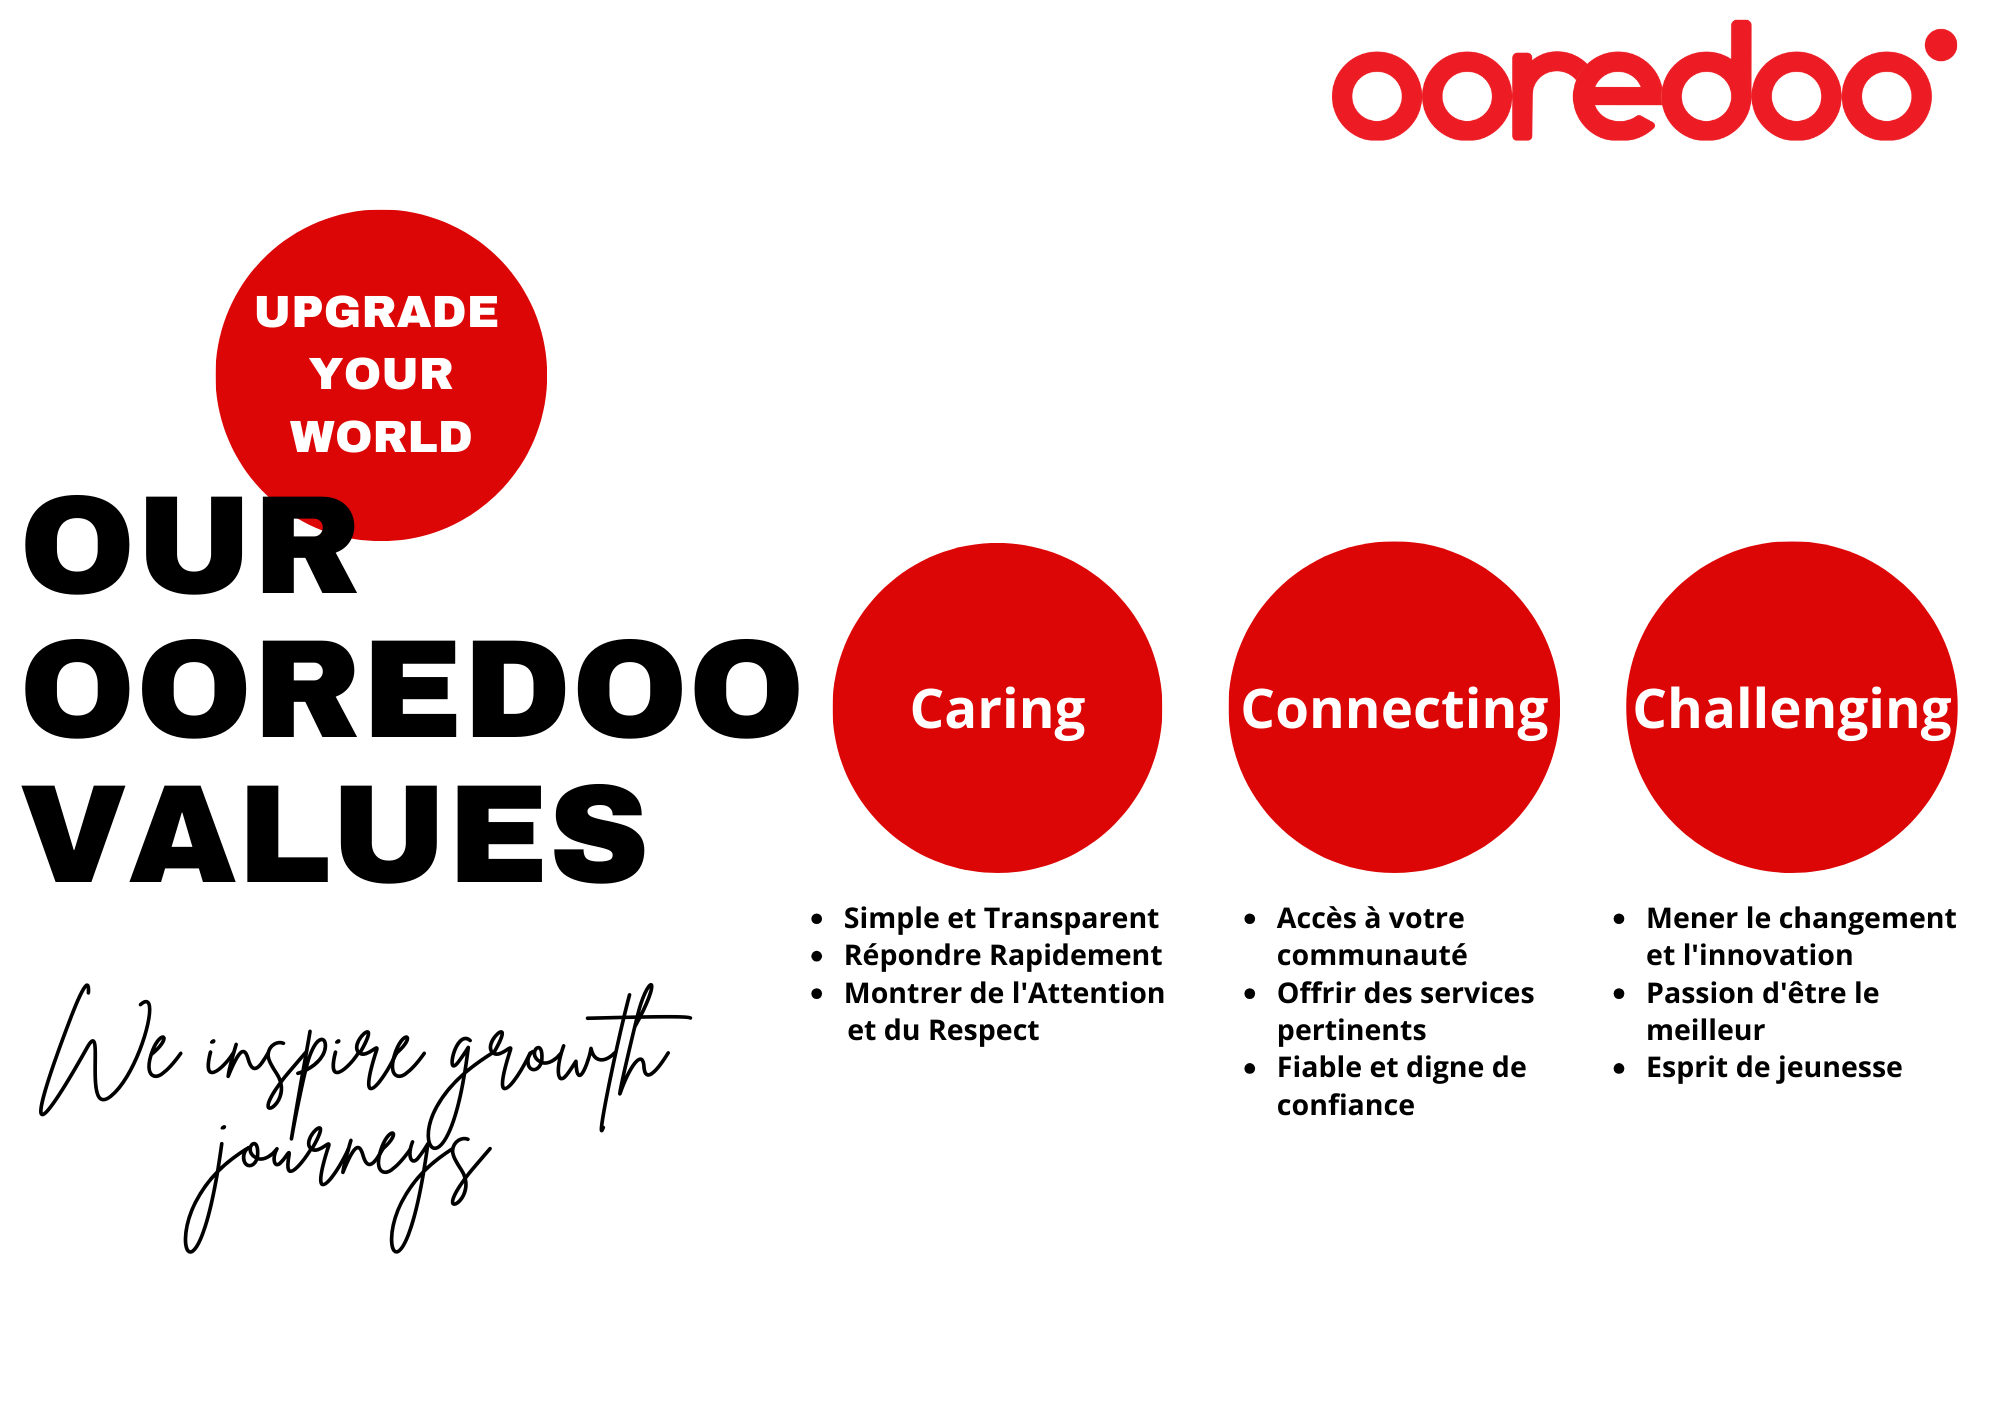
\includegraphics[width=0.6\linewidth]{Value_Ooredoo.png}
    \caption{Récapitulatif des valeurs de l’entreprise}
    \label{valeurs}
\end{figure}

\subsection{La vision de l’entreprise}

 Ooredoo, en tant qu'entreprise résolument orientée vers les besoins des populations, est animée par une vision claire: \textbf{enrichir la vie numérique des gens}. Cette vision repose sur la conviction que la communication est un puissant levier pour stimuler le développement humain et aider les individus à atteindre leurs objectifs, tant personnels que professionnels. 

Ooredoo se donne pour mission de permettre à ses clients d'accéder au meilleur de l'Internet, de manière personnalisée et adaptée à leurs besoins uniques. 

Pour ce faire, l'entreprise continue d'investir dans son réseau Supernet, garantissant des vitesses plus rapides et une connectivité fluide qui répond aux exigences croissantes du monde numérique. 

En tant que véritable facilitateur digital, Ooredoo aspire à simplifier la vie de ses utilisateurs et à leur offrir des expériences numériques enrichissantes et gratifiantes. Prenant les devants dans le domaine des services intelligents, Ooredoo contribue à la construction des « smart cities » et des « smart stadiums » de demain, tout en proposant une riche gamme de services, allant des divertissements numériques à Ooredoo Mobile Money.


\subsection{L’organigramme de l’entreprise} 

 Ooredoo Tunisie compte un effectif total de \textbf{1357 salariés}, comprenant \textbf{838 hommes} et \textbf{519 femmes}.

 Le siège se compose de dix directions, à savoir : Direction des Ressources Humaines, Direction de la Technologie, Direction Administrative et Financière, Direction Vente et Distribution, Direction Marketing et Direction Juridique et Régulation.
 La figure \ref{Hier} ci-dessous montre la répartition des principaux postes de direction au sein de l'entreprise.
\begin{figure}[H]
    \centering
    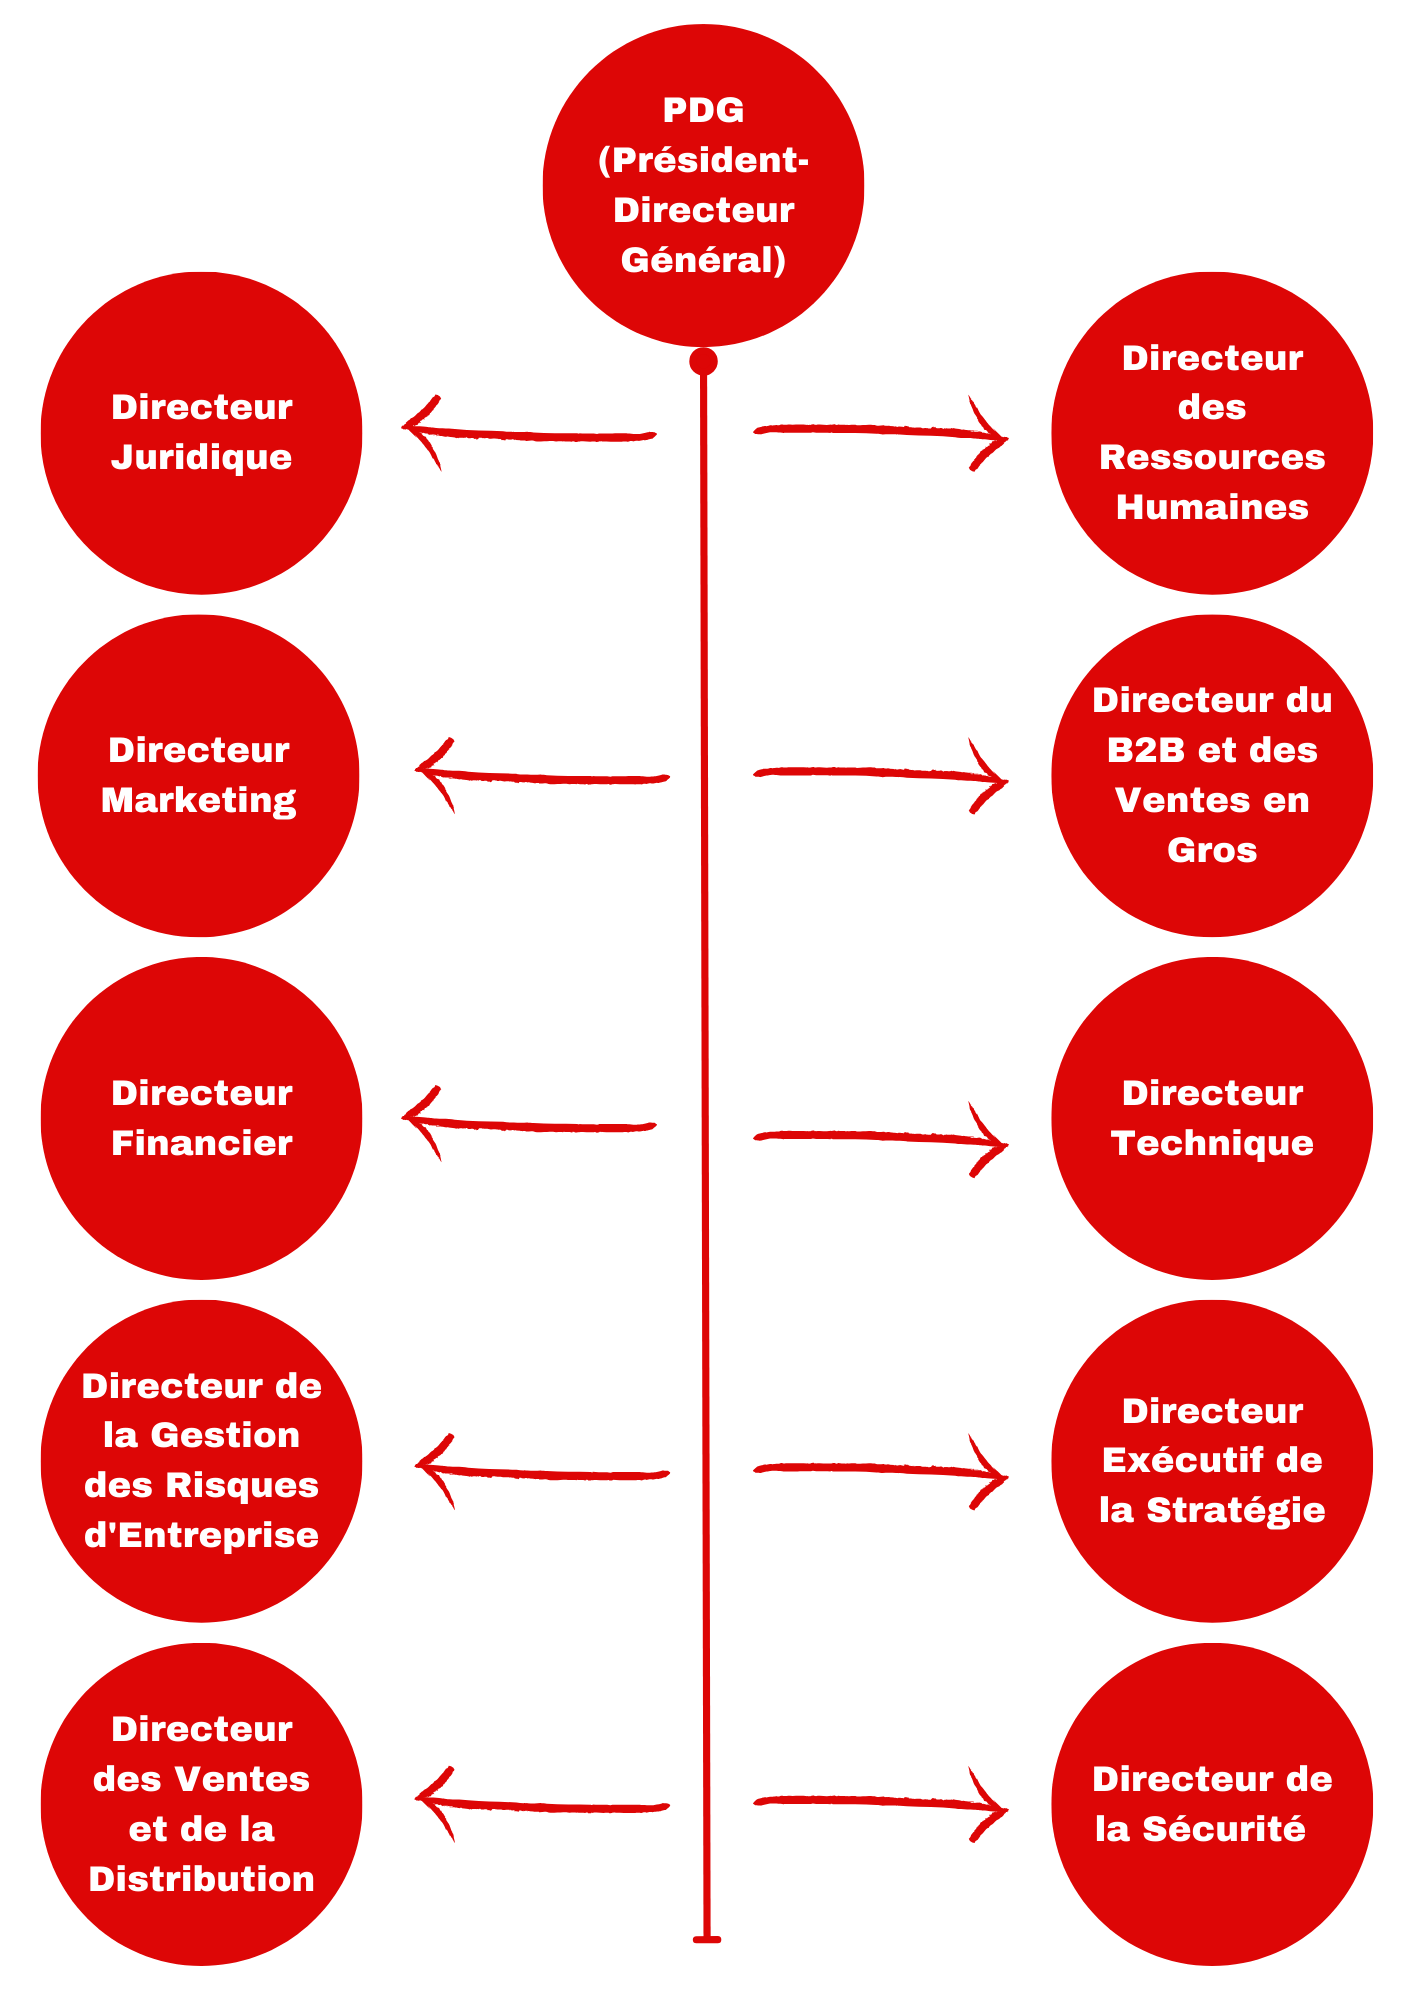
\includegraphics[width=0.5\linewidth]{General_Ooredoo.png}
    \caption{La répartition des principaux postes de direction}
    \label{Hier}
\end{figure}

\subsection{L’organigramme de la direction Technologie }

Au sein de la Direction Technologie d'Ooredoo Tunisie, plusieurs sous-directions jouent un rôle clé dans la gestion et le développement des infrastructures et services technologiques.
La Direction CME (Centre de Maintenance et d'Exploitation) est responsable de la maintenance préventive et corrective des équipements ainsi que de leur exploitation quotidienne pour garantir leur bon fonctionnement. 
\begin{itemize}
    

\item La Direction Support assure l'assistance technique aux utilisateurs internes et externes, gérant les demandes de support et résolvant les problèmes techniques. 
\item La Direction Déploiement et Maintenance se concentre sur l'installation et la configuration des nouvelles solutions technologiques, ainsi que sur la maintenance des systèmes existants. 
\item La Direction Technique est chargée de la gestion des aspects techniques des projets, incluant la conception et l'implémentation de nouvelles technologies. 
\item La Direction Réseau et Service gère l'infrastructure réseau, veillant à la performance et à la sécurité des services de télécommunications. 
\item La Direction Budget, Process et Gestion de Projet supervise la planification budgétaire, les processus internes et le suivi des projets pour assurer leur livraison dans les délais et les coûts impartis.
\item La Direction des Systèmes d'Information (DSI), où se déroule mon stage, est essentielle au sein de la Direction Technologie. Elle s'occupe de la mise en place, du suivi, de la maintenance et de l'optimisation des systèmes informatiques d'Ooredoo. La DSI centralise les données et coordonne des applications clés comme les CRM, ERP, et Data Warehouse, soutenant ainsi les opérations quotidiennes, optimisant les processus internes et facilitant la prise de décision stratégique. Sa gestion est cruciale pour répondre aux besoins croissants en gestion des données et en technologies de l'information.
\end{itemize}

La figure \ref{it} ci-dessous montre la répartition des différentes directions au sein de la direction Technique.
\begin{figure}[H]
    \centering
    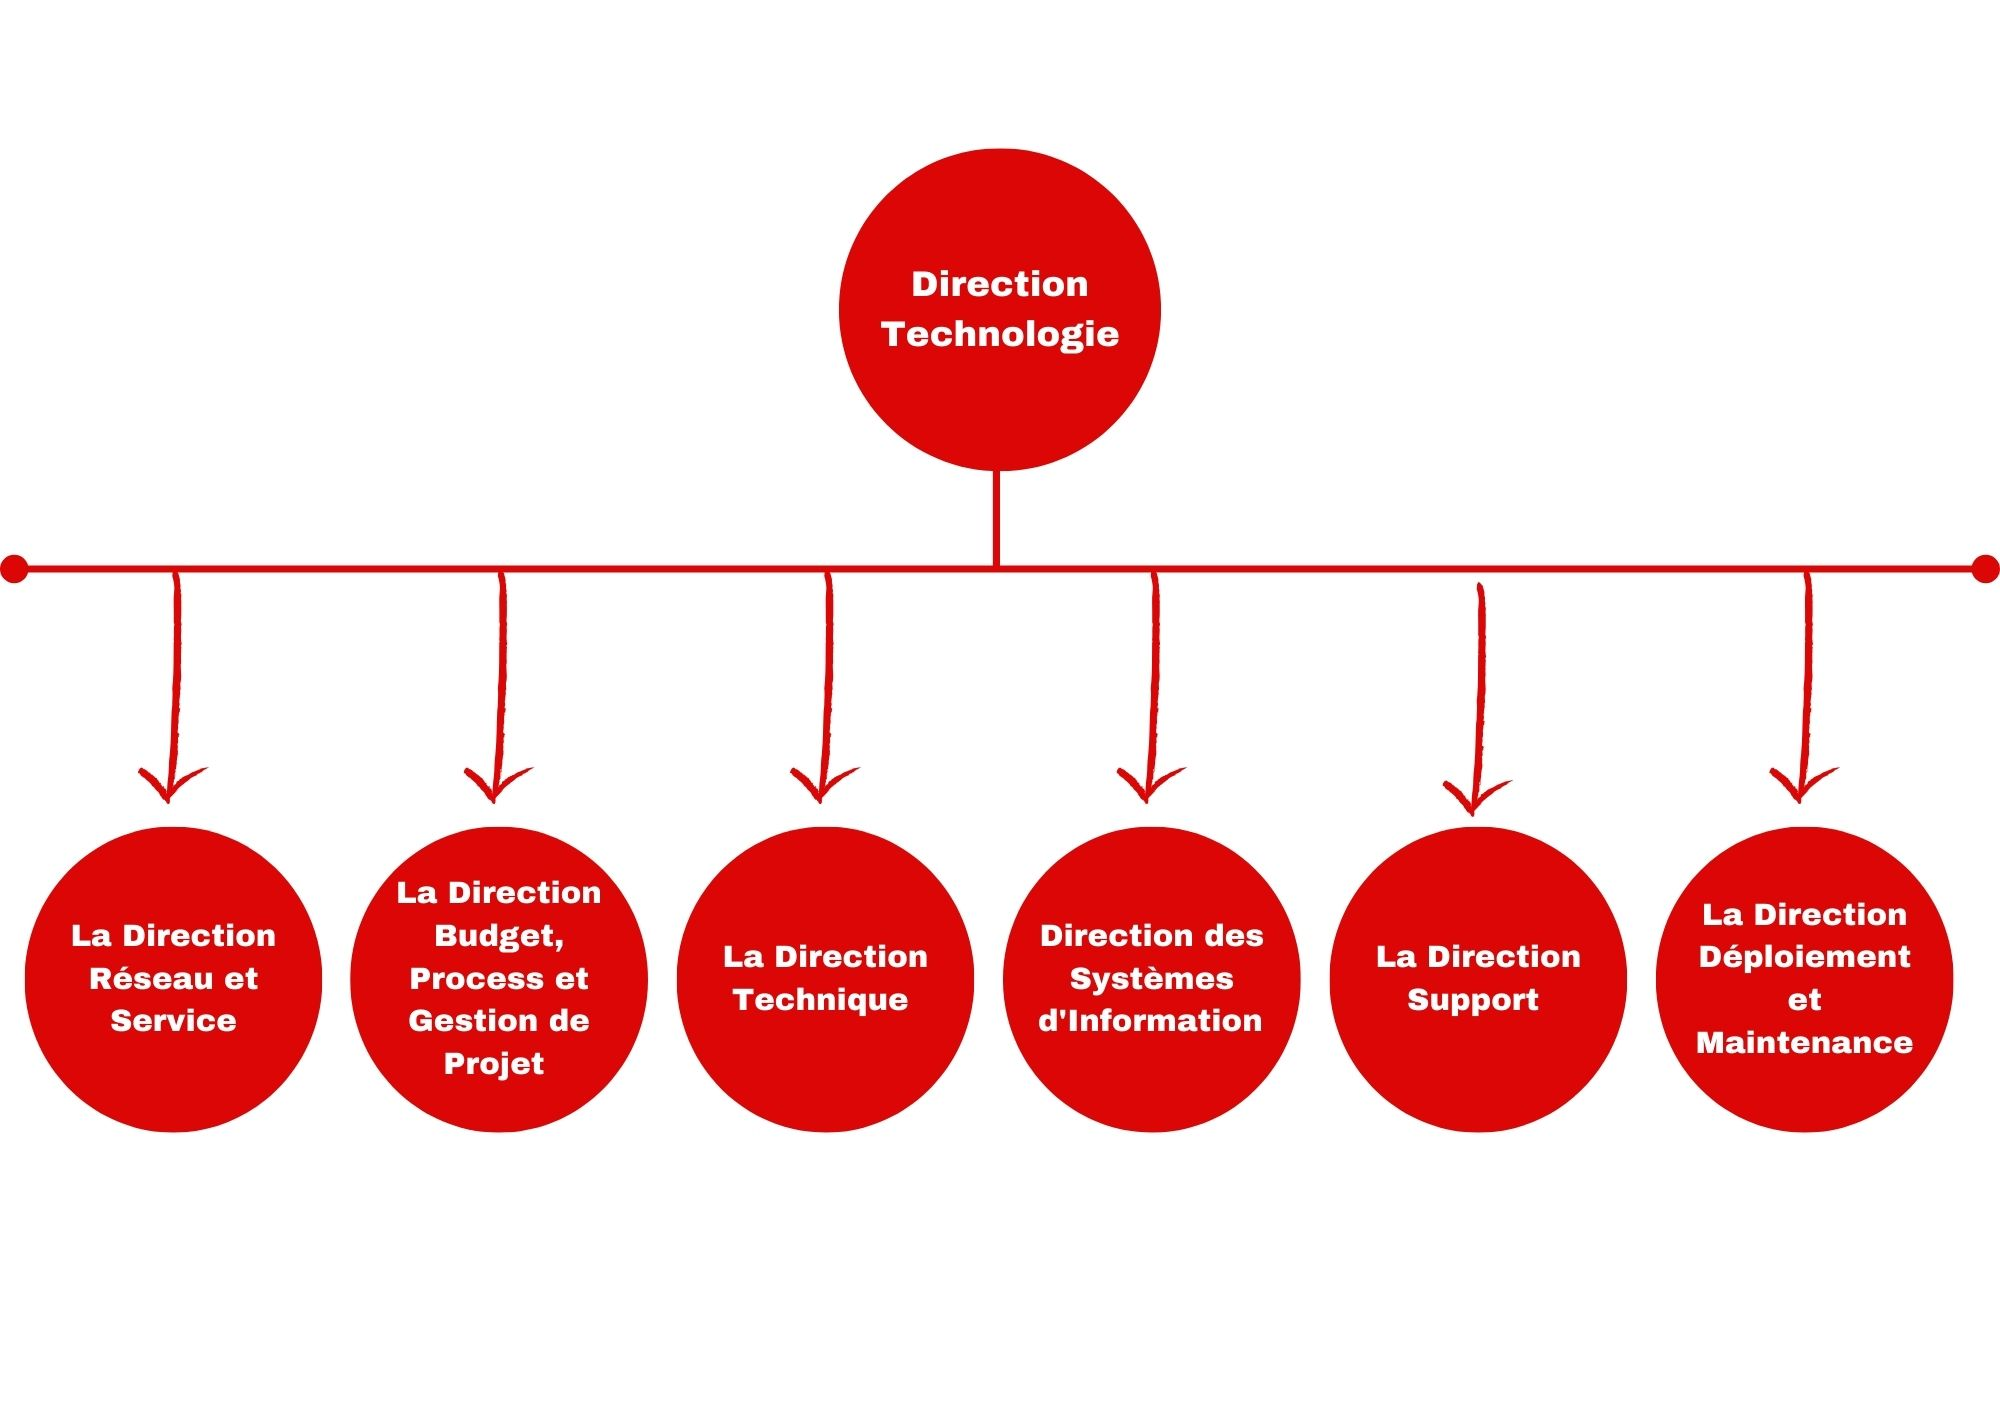
\includegraphics[width=0.5\linewidth]{DepIT_Ooredoo.jpg}
    \caption{Répartition des différentes directions au sein de la direction Technique}
    \label{it}
\end{figure}

\section{Contexte générale du projet}
\subsection{Problématique}

Dans le secteur des télécommunications, la satisfaction des clients est essentielle pour fidéliser la clientèle et se démarquer de la concurrence, notamment face à des acteurs comme Orange et Tunisie Telecom. Les revenus des opérateurs dépendent largement de leur capacité à retenir leurs clients, car l’acquisition de nouveaux clients est souvent plus coûteuse.\par

Comprendre les raisons de la satisfaction ou de l'insatisfaction des clients est donc crucial pour ajuster les stratégies de service et de marketing. Il est important de noter que dans ce secteur, deux types principaux de clients se distinguent : les \textbf{clients prépayés} et les \textbf{clients postpayés}.

\textbf{Clients Prépayés:} Ces clients paient à l'avance pour les services téléphoniques (appels, SMS, données). Leur utilisation dépend de leurs habitudes de consommation et de leur capacité à recharger leur crédit. Ils constituent une catégorie homogène, dont le comportement est influencé par la fréquence et le montant des recharges. Ainsi, les données liées aux recharges, comme \texttt{recharge\_amount} et \texttt{number\_of\_recharges}, sont des indicateurs clés pour comprendre leur satisfaction.
\textbf{Clients Postpayés:} Ces clients, au contraire, paient pour les services utilisés à la fin du mois. Leur consommation est plus stable et moins directement influencée par les recharges. Toutefois, leur comportement est fortement impacté par les offres et promotions auxquelles ils souscrivent, rendant leur analyse plus complexe.

Ces distinctions entre clients prépayés et postpayés sont essentielles pour adapter les analyses et les stratégies de rétention.

En \textbf{2022}, \textbf{Tunisie Telecom} a enregistré un chiffre d’affaires de 1 288,22 millions de dinars, en \textbf{hausse de 2,6\%} par rapport à \textbf{2021}. \textbf{Orange} Tunisie a atteint 773,16 millions de dinars, avec une \textbf{augmentation de 8,8\%}. En revanche, \textbf{Ooredoo} Tunisie, qui avait affiché le plus gros chiffre d’affaires du secteur en 2021 avec 1 351,1 millions de dinars, a vu ce chiffre \textbf{baisser de 0,7\%}, s'établissant à 1 306,40 millions de dinars en 2022. Cette situation met en lumière l'importance de mieux comprendre les attentes des clients pour inverser cette tendance.\par

Ooredoo mène des enquêtes mensuelles sur divers aspects tels que la recharge, le réseau, et le retail, pour analyser le comportement des clients au cours des mois précédents. L'objectif est d'identifier les facteurs qui influencent le score de satisfaction (OSAT) et de développer des modèles prédictifs grâce aux techniques de machine learning et de deep learning.\par

En utilisant ces analyses, Ooredoo peut non seulement repérer les clients à risque de départ, mais aussi anticiper leurs besoins pour améliorer leur expérience. Ce projet vise à renforcer la relation client en exploitant les outils avancés de la data science, essentiels pour rester compétitif sur le marché.\par

Pour répondre à cette problématique, ce projet s'efforcera de répondre aux questions suivantes:

\begin{itemize}
    \item Quels sont les principaux facteurs qui influencent la satisfaction des clients ?
    \item Quelles différences de comportement peut-on observer entre les clients satisfaits et insatisfaits, notamment entre les clients prépayés et postpayés ?
    \item Quels modèles de machine learning ou de deep learning offrent les meilleures performances pour prédire la satisfaction générale des clients ?
\end{itemize}

\subsection{Objectif du projet}

L'objectif principal de ce projet est d'explorer et d'analyser les données clients pour comprendre les facteurs influençant leur satisfaction. En se concentrant principalement sur les \textbf{clients prépayés}clients prépayés, ce projet vise à :

\begin{itemize}
    \item \textbf{Identifier les principaux facteurs} qui influencent la satisfaction ou l'insatisfaction des clients.
    \item \textbf{Distinguer les comportements} entre clients satisfaits et insatisfaits en analysant les réponses aux enquêtes et les comportements d’utilisation des services.
    \item \textbf{Développer des modèles prédictifs} utilisant des techniques de machine learning et de deep learning pour prédire avec précision le score de satisfaction (OSAT).
    \item \textbf{Optimiser l’expérience client} en identifiant les segments nécessitant des améliorations spécifiques, notamment par une analyse approfondie des clients prépayés.
\end{itemize}

Le projet se déroulera en plusieurs phases : la collecte et le nettoyage des données, l’analyse des résultats, le développement et l’évaluation de modèles prédictifs, ainsi que l'interprétation des résultats pour une application directe dans les stratégies marketing.
\subsection{Méthodologie de travail}

Pour mener à bien ce projet, une approche méthodologique structurée est essentielle. La démarche se décline en plusieurs étapes clés:

\begin{enumerate}
    \item \textbf{Compréhension de la problématique métier}: Cette phase consiste à analyser les enjeux de la satisfaction client dans les télécommunications, à définir les objectifs du projet et à identifier les critères de succès pour Ooredoo Tunisie.
    
    \item \textbf{Compréhension des données}: Cette étape inclut la collecte des données à partir des enquêtes mensuelles d'Ooredoo, suivie de leur nettoyage, transformation et préparation pour garantir leur qualité et pertinence pour l'analyse.
    
    \item \textbf{Analyse des variables}: Cette phase comprend l'exploration des relations entre les variables explicatives et la variable cible (score de satisfaction) en utilisant des techniques telles que la corrélation. Cette analyse permet d'identifier les facteurs influents, leurs interactions et leur impact sur la satisfaction des clients.
    
    \item \textbf{Modélisation}: Nous utilisons divers algorithmes de machine learning et deep learning pour créer des modèles prédictifs. Cette étape vise à développer des modèles capables de prédire avec précision le score de satisfaction des clients.
    
    \item \textbf{Évaluation du modèle}: Après la modélisation, chaque modèle est évalué en termes de performance à l'aide de métriques telles que l'exactitude, la précision, le rappel et le F1-score. Cette évaluation permet de sélectionner le modèle le plus performant.
\end{enumerate}

\subsection{Choix technologiques}

Pour réaliser les différentes étapes du projet, plusieurs outils technologiques ont été sélectionnés. Ces outils peuvent être classés en trois catégories: logiciels et environnements de développement, langages de programmation et bibliothèques.

\begin{itemize}
    \item \textbf{Logiciels et environnements de développement}  
    \begin{itemize}
        \item \textbf{SAS Viya}: Une plateforme analytique puissante permettant l'accès aux données, leur manipulation et l'exécution de requêtes complexes en SQL. Utilisée principalement pour manipuler les tables de données et exporter les résultats finaux pour l'analyse.
        \item \textbf{Jupyter Notebook}: Un environnement de développement interactif combinant code, texte et visualisations dans un même document, particulièrement adapté à l'analyse exploratoire des données et la modélisation prédictive.   
    \end{itemize}
    \item \textbf{Langages de programmation}  
    \begin{itemize}
        \item \textbf{Python}: Langage polyvalent largement utilisé dans l'analyse de données, la modélisation statistique et le machine learning. Il permet de réaliser des tâches complexes grâce à ses bibliothèques variées.
        \item \textbf{SQL}: Langage utilisé pour interagir avec les bases de données relationnelles, permettant d'extraire, manipuler et gérer des ensembles de données.
    \end{itemize}
    \item \textbf{Bibliothèques utilisées}  
    \begin{itemize}
        \item \textbf{Numpy}: Bibliothèque fondamentale pour le calcul numérique, permettant de manipuler des tableaux multidimensionnels et de réaliser des opérations mathématiques complexes.
        \item \textbf{Pandas}: Bibliothèque spécialisée dans la manipulation et l'analyse de données, offrant des structures flexibles pour le nettoyage et la transformation des données.
        \item \textbf{Matplotlib}: Bibliothèque de visualisation pour créer des graphiques statiques en 2D.
        \item \textbf{Seaborn}: Basée sur Matplotlib, elle simplifie la création de graphiques statistiques et propose des styles graphiques avancés.
        \item \textbf{Scikit-learn}: Fournit une large gamme d'algorithmes pour la classification, la régression, le clustering et la réduction de dimension.
        \item \textbf{TensorFlow}: Bibliothèque open source pour créer et entraîner des modèles de machine learning, notamment des réseaux de neurones.        \item \textbf{Keras}: Interface de haut niveau pour simplifier la création et la manipulation de réseaux de neurones profonds.
        \item \textbf{PyTorch}: Bibliothèque open source de Facebook, largement utilisée pour la recherche en deep learning.    \end{itemize}
\end{itemize}

\section{Concepts Clés}
L'ère numérique a révolutionné l'exploitation des données. Dans ce contexte, le Machine Learning, le Data Mining et le Deep Learning jouent un rôle clé pour analyser les données massives et en extraire des insights significatifs. 

Le Data Mining permet d'explorer et de découvrir des modèles dans les données, tandis que le Machine Learning utilise ces insights pour construire des modèles prédictifs. Enfin, le Deep Learning, en tant que sous-domaine du Machine Learning, emploie des réseaux de neurones profonds pour traiter des données non structurées et capturer des relations complexes.

Cette section abordera chacun de ces concepts, en soulignant leur définition et leur application dans le projet de prédiction de la satisfaction client.

\subsection{Data Mining}

Le \textbf{Data Mining}, ou fouille de données, est le processus d'analyse de grandes quantités de données pour découvrir des informations utiles, des tendances cachées, ou des relations insoupçonnées. Utilisé dans divers secteurs comme le marketing, la santé, ou l'éducation, il permet aux entreprises de mieux comprendre leurs clients et d'optimiser leurs stratégies en fonction des comportements observés.

Contrairement à d'autres approches, le Data Mining se concentre surtout sur l'analyse exploratoire des données, visant principalement la découverte de connaissances sans passer par une phase de prédiction.
Les principales étapes du processus de Data Mining sont les suivantes:

\begin{itemize}
    \item \textbf{Collecte des données}: Rassemblement d'informations à partir de diverses sources, telles que des bases de données ou des fichiers.
    \item \textbf{Préparation des données}: Nettoyage et transformation des données afin d'assurer leur qualité, en supprimant les erreurs, en gérant les valeurs manquantes, et en normalisant les variables. Cette phase inclut également des techniques comme le \textbf{clustering} pour regrouper les données en sous-ensembles homogènes, facilitant ainsi leur analyse. Dans certains cas, des méthodes comme \textbf{SMOTE} (Synthetic Minority Over-sampling Technique) peuvent être utilisées pour rééquilibrer les jeux de données déséquilibrés.
    \item \textbf{Exploration des données}: Utilisation d'outils statistiques et analytiques pour identifier des tendances, des motifs ou des anomalies.
\end{itemize}


Le Data Mining applique des techniques comme le clustering et la classification pour explorer les données, avec un objectif surtout descriptif, contrairement aux approches prédictives du Machine Learning. Il permet ainsi de comprendre les données, découvrir des corrélations, et faciliter des décisions éclairées.
\subsection{Machine Learning}

Le \textbf{Machine Learning}, ou apprentissage automatique, est une branche de l'intelligence artificielle (IA) qui permet aux machines d'apprendre à partir de données sans être explicitement programmées pour chaque tâche. Contrairement au Data Mining, le Machine Learning est principalement orienté vers la prédiction et l'automatisation de tâches à partir de modèles qui apprennent continuellement à partir des données.

Il existe trois principaux types de Machine Learning:

\begin{itemize}
    \item \textbf{Apprentissage supervisé}: Le modèle apprend à partir de données étiquetées, où les entrées sont associées à des sorties connues. Exemple: prédire la satisfaction des clients en fonction de caractéristiques passées.
    \item \textbf{Apprentissage non supervisé}: Le modèle identifie des structures cachées dans les données non étiquetées. Exemple: regrouper des clients en fonction de comportements similaires via le \textbf{clustering}.
    \item \textbf{Apprentissage par renforcement}: Le modèle interagit avec un environnement et apprend à partir des récompenses ou pénalités qu'il reçoit. Cette approche est souvent utilisée dans des applications comme la robotique ou les jeux vidéo.
\end{itemize}

Le Machine Learning se distingue du Data Mining par son caractère itératif et automatisé. Une fois que le modèle est entraîné, il peut faire des prédictions sur de nouvelles données et s'améliorer au fil du temps. Le processus typique de Machine Learning comprend les étapes suivantes:

\begin{itemize}
    \item \textbf{Sélection des caractéristiques}: Identification des variables clés pour l'entraînement des modèles.
    \item \textbf{Choix des algorithmes}: En fonction des objectifs, différents algorithmes comme la \textbf{régression logistique}, les \textbf{forêts aléatoires} ou les \textbf{SVM} sont utilisés.
    \item \textbf{Entraînement du modèle}: Le modèle est ajusté à l'aide de données d'entraînement pour minimiser l'erreur entre les prédictions et les résultats réels.
    \item \textbf{Évaluation et optimisation}: Le modèle est évalué et amélioré à l'aide de techniques comme la validation croisée et l'optimisation des hyperparamètres.
\end{itemize}

\subsection{Data Mining vs Machine Learning}

Bien que le \textbf{Data Mining} et le \textbf{Machine Learning} partagent des outils et objectifs, comme l'exploration des données pour extraire des informations utiles, leurs approches et finalités diffèrent:
\begin{itemize}
    \item Le \textbf{Data Mining} est principalement orienté vers l'exploration et la compréhension des données historiques à l'aide de techniques descriptives. Il est souvent utilisé pour découvrir des modèles et des relations au sein des données.
    \item Le \textbf{Machine Learning}, quant à lui, adopte une approche prédictive et automatisée. Il vise à créer des modèles capables de généraliser à de nouvelles données pour prédire des résultats futurs.
    \item Dans le Data Mining, les techniques comme la \textbf{classification} et le \textbf{clustering} sont utilisées pour segmenter les données et en extraire des connaissances. En Machine Learning, ces mêmes techniques sont utilisées pour construire des modèles prédictifs qui évoluent au fil du temps.
\end{itemize}


En somme, bien que complémentaires, le Data Mining et le Machine Learning diffèrent dans leurs applications. Le Data Mining s'attache à décrire et analyser les données existantes, tandis que le Machine Learning se concentre sur l'automatisation et la prédiction, permettant de prendre des décisions ou d'effectuer des tâches complexes à grande échelle.

\subsection{Deep Learning}

Le \textbf{Deep Learning} est une branche spécifique du Machine Learning qui repose sur l'utilisation de réseaux de neurones artificiels. Contrairement aux algorithmes de Machine Learning traditionnels, les modèles de Deep Learning peuvent apprendre à partir de grandes quantités de données non structurées et extraire automatiquement des caractéristiques complexes sans intervention humaine. 

Ce processus est particulièrement efficace dans des domaines comme la reconnaissance d'images, le traitement du langage naturel, et l'analyse vocale, où les données sont volumineuses et hétérogènes.

Les réseaux de neurones artificiels utilisés en Deep Learning sont composés de plusieurs couches d'unités (ou neurones) qui sont interconnectées. Les modèles les plus communs sont les réseaux de neurones à propagation avant (feedforward) et les réseaux de neurones convolutifs (CNN) pour les images.

\subsubsection{Principes du Deep Learning}

Le Deep Learning se distingue par sa capacité à apprendre des représentations complexes à travers les couches hiérarchiques des réseaux de neurones:

\begin{itemize}
    \item \textbf{Les couches de neurones}: Un réseau de neurones profond est composé de plusieurs couches successives. Chaque couche transforme les données reçues, en extrayant des caractéristiques de plus en plus abstraites.
    \item \textbf{Fonctions d'activation}: Chaque neurone utilise une fonction d'activation (comme \textbf{ReLU}, \textbf{sigmoïde} ou \textbf{tanh}) pour introduire de la non-linéarité, permettant ainsi au modèle d'apprendre des relations complexes dans les données.
    \item \textbf{Entraînement par rétropropagation}: Les réseaux de neurones sont entraînés à l'aide d'une technique appelée \textbf{backpropagation}, qui ajuste les poids des connexions entre les neurones en minimisant une fonction de coût via la descente de gradient.
    \item \textbf{Régularisation et Dropout}: Pour prévenir le sur-apprentissage (overfitting), des techniques telles que la régularisation L2 ou le \textbf{dropout} sont appliquées. Le dropout désactive aléatoirement des neurones pendant l'entraînement pour améliorer la généralisation.
\end{itemize}

\subsubsection{Applications du Deep Learning}

Le Deep Learning est particulièrement adapté pour les tâches impliquant de grandes quantités de données non structurées. Voici quelques exemples d'applications:

\begin{itemize}
    \item \textbf{Reconnaissance d'images}: Utilisation des réseaux de neurones convolutifs (CNN) pour identifier des objets, visages ou scènes dans les images.
    \item \textbf{Traitement du langage naturel (NLP)}: Utilisation de modèles tels que les \textbf{réseaux de neurones récurrents (RNN)} ou les \textbf{transformers} pour la traduction, la génération de texte, ou l'analyse des sentiments.
    \item \textbf{Analyse vocale}: Reconnaissance vocale automatisée via des réseaux profonds pour transformer les signaux audio en texte ou en commandes.
\end{itemize}

\subsubsection{Différence entre Machine Learning et Deep Learning}

Le Deep Learning, sous-catégorie du Machine Learning, se distingue par sa capacité à traiter de grandes quantités de données et à extraire automatiquement des caractéristiques complexes sans intervention manuelle.
Voici quelques différences principales:
\begin{itemize}
    \item \textbf{Caractéristiques automatiques}: Contrairement au Machine Learning traditionnel où les ingénieurs sélectionnent manuellement les caractéristiques, en Deep Learning, les modèles apprennent automatiquement à extraire les meilleures caractéristiques des données brutes.
    \item \textbf{Quantité de données}: Le Deep Learning nécessite généralement beaucoup plus de données pour fonctionner efficacement, alors que les algorithmes de Machine Learning traditionnels peuvent être appliqués à des ensembles de données plus petits.
    \item \textbf{Complexité des modèles}: Les modèles de Deep Learning, composés de nombreuses couches de neurones, sont bien plus complexes et peuvent capturer des relations non linéaires plus profondes que les modèles de Machine Learning classiques.
\end{itemize}

Ainsi, le Deep Learning permet de traiter des problèmes complexes nécessitant un apprentissage à partir de données massives et non structurées, offrant des performances exceptionnelles dans des domaines comme la vision par ordinateur et le traitement du langage naturel.

\section{Conclusion}
Ce chapitre a posé les bases nécessaires à la compréhension du projet en détaillant son contexte, ses objectifs, et les concepts théoriques associés. Les éléments présentés permettront de mieux appréhender les étapes suivantes de l'analyse et de la modélisation des données dans les prochains chapitres.
